As stated in \Cref{sub:technologies}, the entire backend of the system is
developed using the Node.js runtime, the TypeScript language, and the NestJS
framework. Following the specifications outlined in \Cref{sec:tool_design},
both the backend and the tool adapter components are monolithic applications.

These components communicate through a message broker, utilising Redis as the
underlying technology for message queuing and delivery. This messaging system
enables seamless interaction and data exchange between the backend and the tool
adapter, facilitating the flow of information within the system's
infrastructure.

\Cref{fig:decomposition_lifecycle} contains the entire decomposition workflow
since the user requests a decomposition for a given tool, until it receives the
result.

\begin{figure*}[!htb]
  \centering
  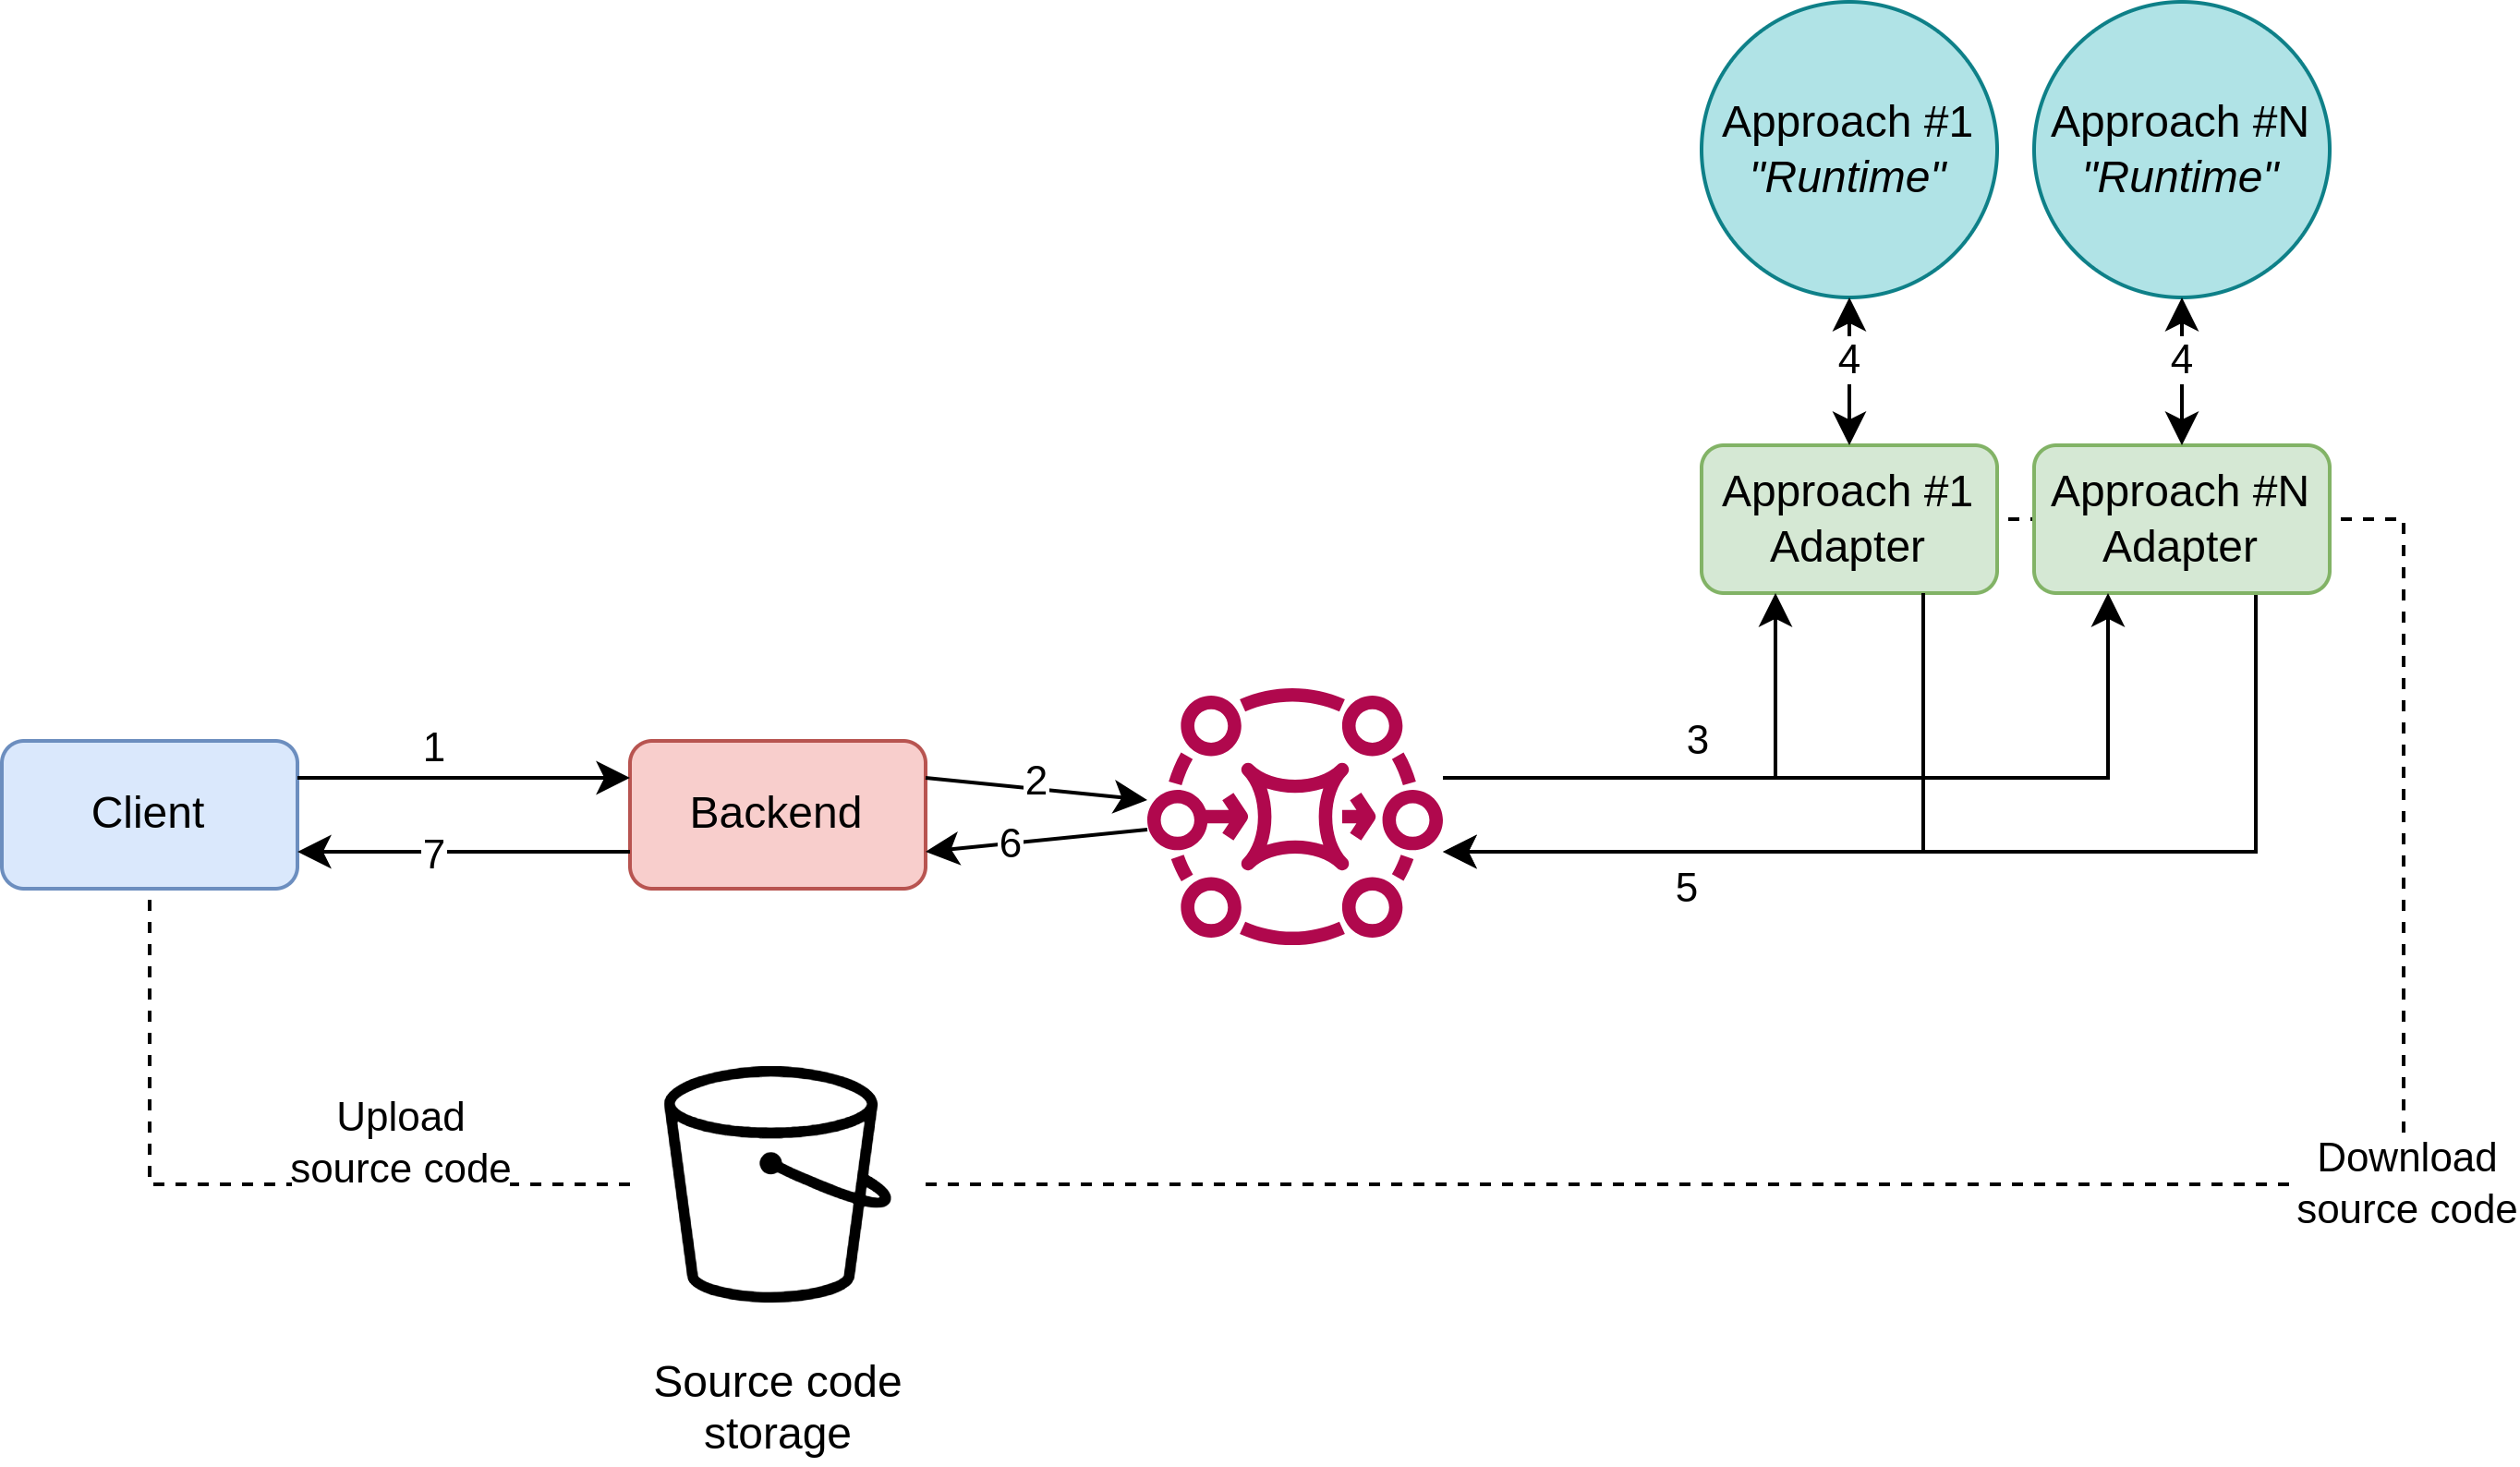
\includegraphics[width=\textwidth]{thesis-architecture-tool-domain.drawio}
  \caption{Decomposition Lifecycle}
  \label{fig:decomposition_lifecycle}
\end{figure*}

\begin{enumerate}
  \item Client uploads (FR05) the project alongside the tools it want to use
    for decomposition.
  \item The backend signals each tool adapter (FR11, FR14) that matches the
    client's request with the unique identifier for that decomposition result
    as well as the identifier of the client's project on S3. This means the
    backend is free to handle new requests (FR10).
  \item Each separate tool adapter (FR16) receives the unique identifier and
    starts an internal job for decomposition.
  \item Each separate tool adapter (FR16) receives the unique identifier and
    starts an internal job for decomposition.
  \item Upon finishing, each tool signals the backend (FR18) about the results,
    that are either success or failure.
  \item When the backend receives the results from each tool adapter, it
    updates the database with the results so that it can always be accessible.
  \item In the end, the backend reports back to the client with the status of
    the result (FR13).
\end{enumerate}
